\section{Shop}
\label{shop}
\label{sec:shop}

\begin{figure}[ht]
	\centering
  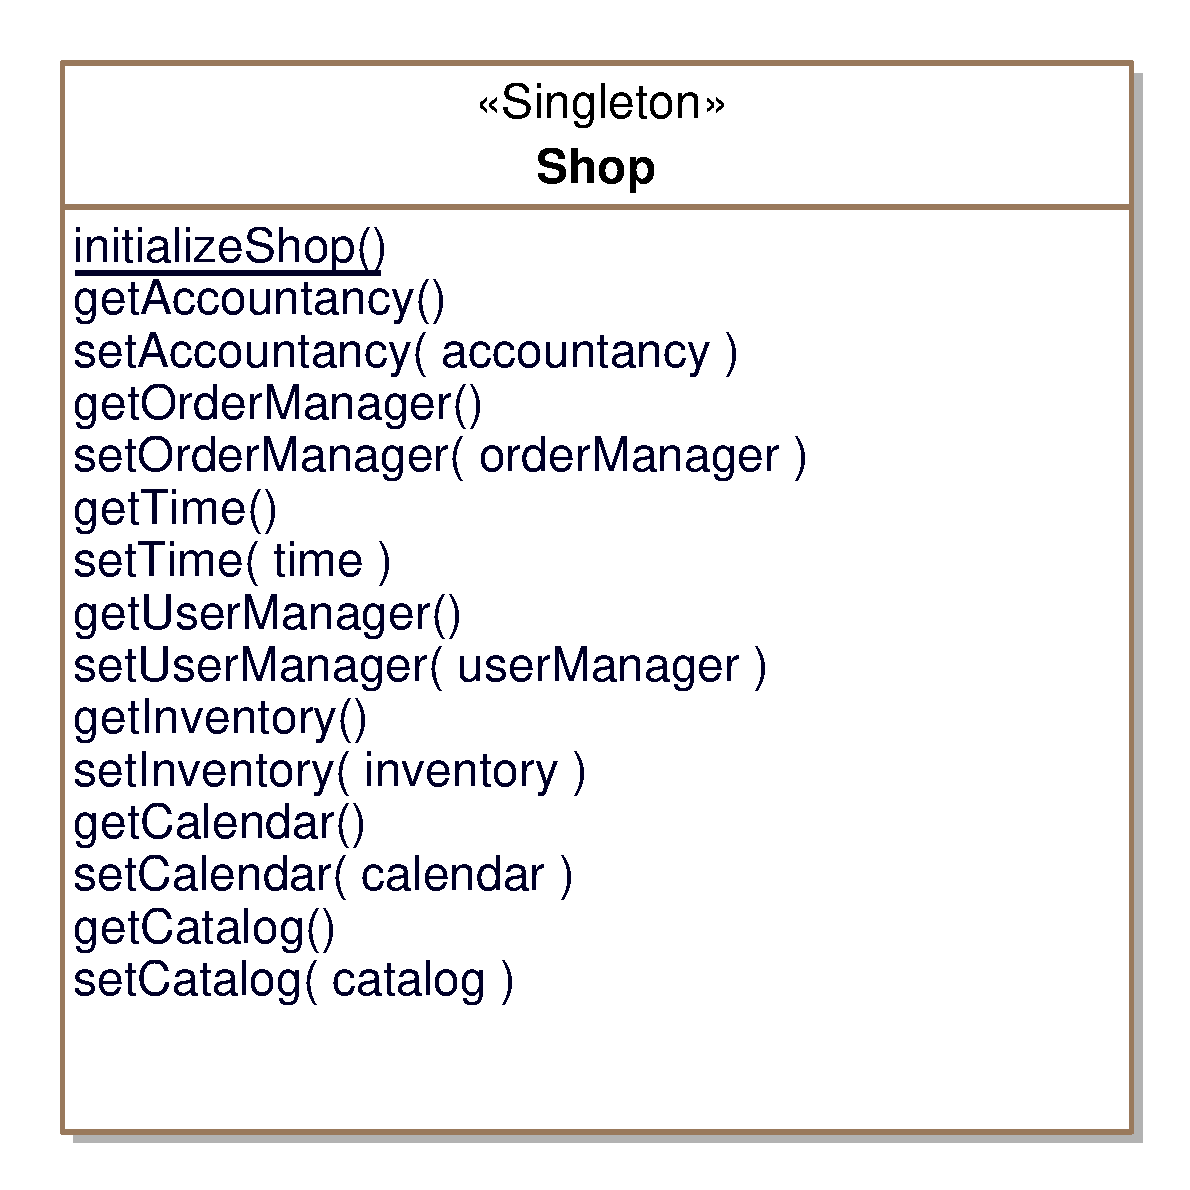
\includegraphics[width=0.45\textwidth]{images/Shop_Overview.eps}
	\label{shop_overview}
	\caption{Shop - Class Overview}
\end{figure}
%TODO reference figure.
%\subsection{\code{Shop} - Starting your SalesPoint-application}
\code{Shop} is a central class in \salespoint{}; it holds references to all manager interfaces and a reference to the \code{Time} interface.
There are six manager interfaces and interfaces aggregating (persistent) objects in \salespoint{}: Accountancy, Calendar, Catalog, Inventory, OrderManager and UserManager.
Other classes use the \code{Shop} to access the manager interfaces, for example \code{Order.completeOrder()} uses \code{Shop.INSTANCE.getInventory()} for product removal.
\code{PersistentCalendar} uses \code{Shop.INSTANCE.getTime()} for time based operations.
There is also a convenience method to minimize boilerplate code\footnote{
	It was mentioned to us, that boilerplate code may also be called infrastructure code.
	We disagree, because we consider configuration files, (startup-) scripts, deployment scripts, etc infrastructure code.
	Wikipedia defines boilerplate code as follows:
	\begin{quote}
		In computer programming, boilerplate is the term used to describe sections of code that have to be included in many places with little or no alteration.
		It is more often used when referring to languages which are considered verbose, i.e. the programmer must write a lot of code to do minimal jobs.
	\end{quote}}
\code{Shop.initializeShop()};
it is used for setting all managers of \code{Shop} to Salespoints persistent class implementations and the time to \code{DefaultTime}.
This behaviour is also known as \textit{convention over configuration}, which means reasonable default values are supplied, eliminating the need to explicitly specify those values in most cases.
\code{Shop} is implemented as a singleton.

Although \code{Shop} holds a references to all managers and aggregating classes (see Section \ref{chap:components}), persistent implementations do not need to be singletons and are infact not.
Moreover, a peculiarity of all managers and aggregating classes is, that a new instance can be created whenever one is needed.
The reason for this behaviour is, that data is not stored inside the manager object itself, as it may be done with a collection-based implementation, but the manager class is merely a transparent interface to the JPA and database.\\


